%\chapter{Análise dos Dados}\label{chapter5}
%pesquisar alguma coisa sobre dados e GA só pra formular uma intro
\section{Earthquake data}
The goal of this research is to find existing patterns in the occurrence of earthquakes. For that it is essential to access trustful data and to explore its details. From the  {\it Japan Meteorological Agency} web page we obtained earthquake data about quakes in Japan. In this data there are information about earthquakes that happened in or nearby Japan,  with the variables: time of the occurrence, magnitude, latitude and longitude and epicentre profundity, for the years of 2000 to 2013.\\

From our first analysis, we discovered a higher number of occurrences of earthquakes during the year of 2011, when the 9.0 $M_w$ earthquake happened, see section~\ref{chapter1}. This earthquake triggered too many after quakes (also called after-shocks) in all Japan. It is considered that big earthquakes may cause others quakes~\cite{zhuang2004analyzing}. In~Figure \ref{ocorrenciasAno} it is possible to visualise a great number of quakes for the year of 2011. Because of this abnormal behaviour and because we decided to focus on more stable occurrences, we limited the tranning base to earthquakes until 2010.\\

\begin{figure}[!htb]
\centering
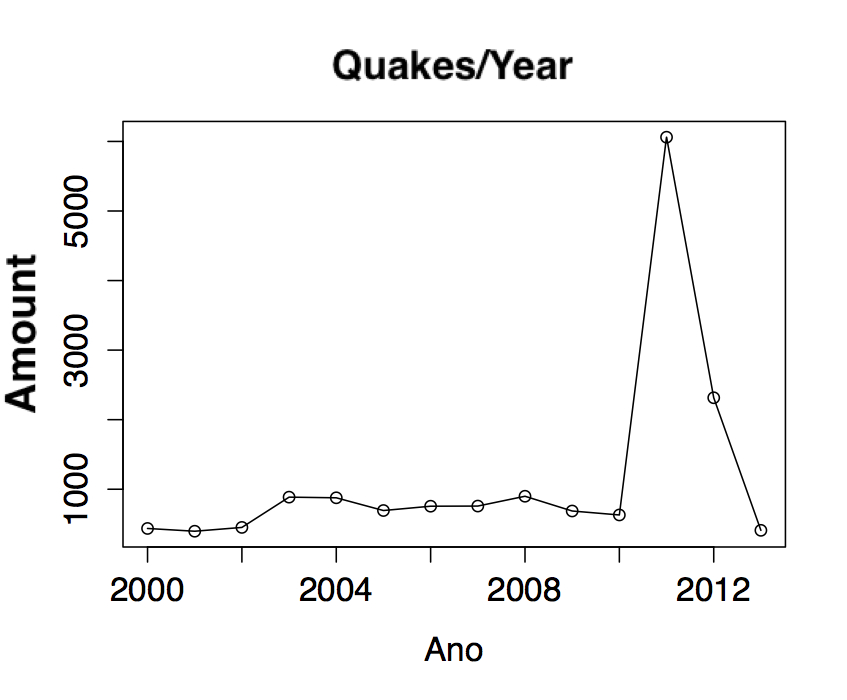
\includegraphics[scale=0.5]{img/ocorrenciasAno.png}
\caption{Amount of earthquake by year.}
\label{ocorrenciasAno}
\end{figure}

Based on the statement done before and considering that we want earthquakes that follow more stable patterns, we selected the ones that happened in land areas or very shallow sea areas, with maximum depth of 100km.\\

\section{Regions}
For the experiments, the data was changed into slices for every year. Each slice is as follows: if the base contains data about a time interval of 10 years, it will be split in 10 slices.\\

We also selected some sub-areas in Japan to better extract and understand earthquakes characteristics and patterns. Those areas are Kanto, Kansai, Touhoku and East Japan. The Figure~\ref{alljapan} shows how we defined them. 

\begin{figure}[H]
	\centering
	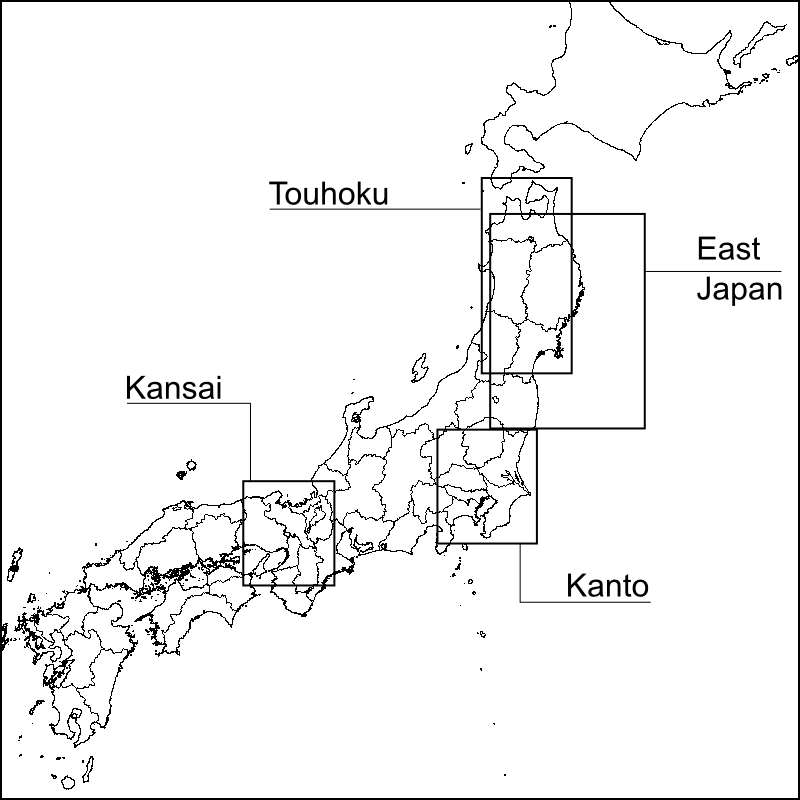
\includegraphics[scale=0.4]{alljapan.png}
	\caption{Japan and the areas used in this studied.}
	\label{alljapan}
\end{figure}


They are described as follows:

\paragraph{Kanto} Kanto is the region around Tokyo. It is area with high seismologic activity during the years we studied. Its coordinates are 34.8 North, 138.8 West, with  2025 bins. Each bin covers an area of approximately 25km$^2$.\\

\begin{figure}[H]
	\centering
	\fbox{
		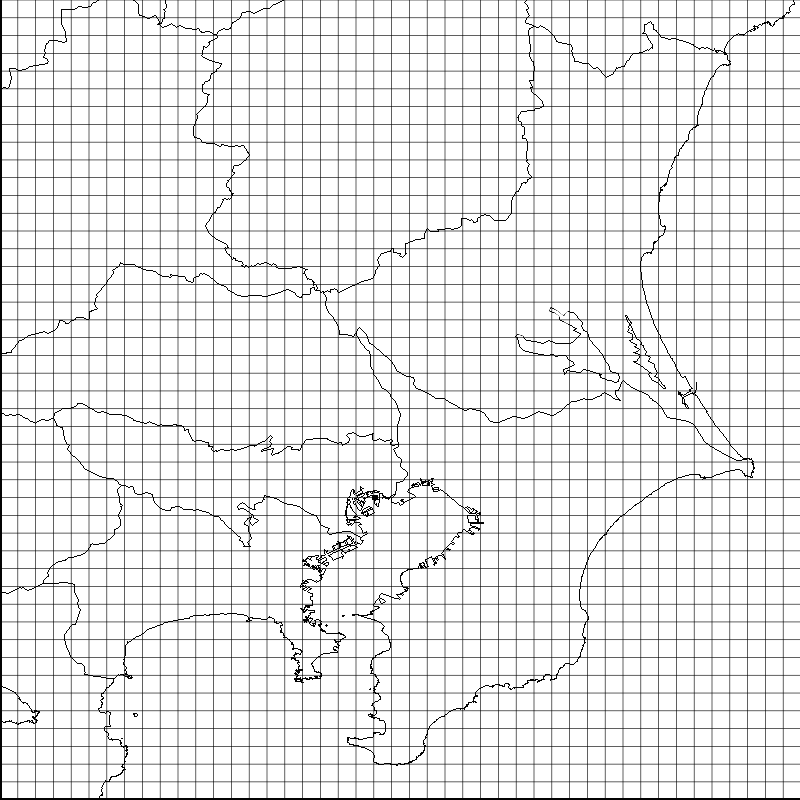
\includegraphics[scale=0.13]{kantomap.png}
	}
	\caption{Japan and the areas used in this studied.}
	\label{kanto}
\end{figure}


\paragraph{Kansai} Kansai is the region that includes Kyoto, Osaka and many others historical cities. In this area, rather than Kanto area, there is a small seismic activity. Its coordinates are 34 North, 134.5 West, with 1600 bins. Each bin covers an area of approximately 25km$^2$.\\

\begin{figure}[H]
	\centering
	\fbox{
		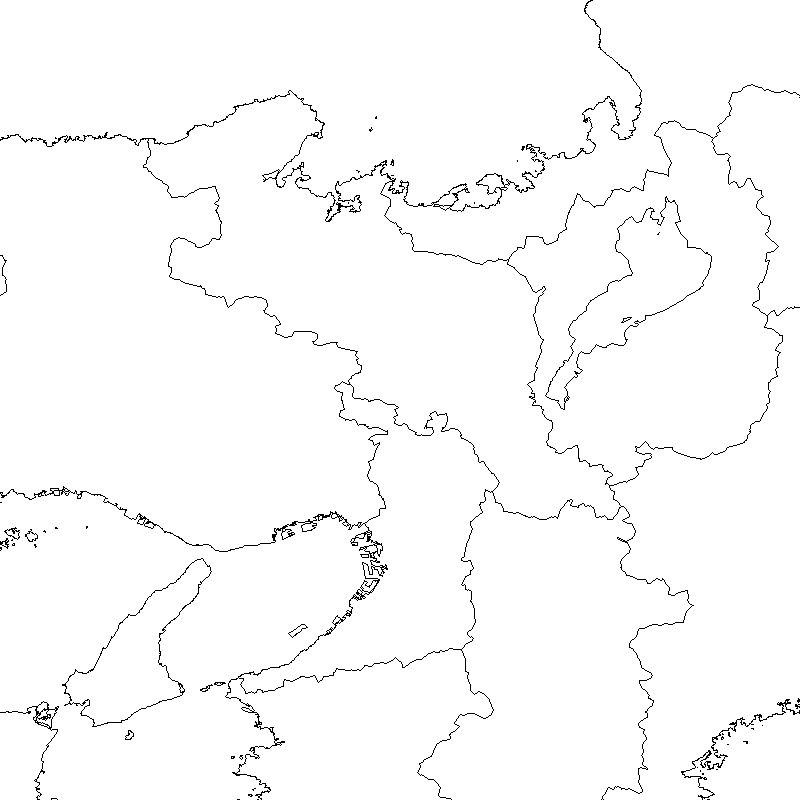
\includegraphics[scale=0.1]{kansai.png}
	}
	\caption{Kansai.}
	\label{kansai}
\end{figure}



\paragraph{Touhoku} Touhoku is the region in the North of the main Japanese island. It has some clusters of seismic activities during the the years we studied. Its coordinates are 37.8 North, 139.8 West, with  800 bins. Each bin covers an area of approximately 100km$^2$. \\

\begin{figure}[H]
	\centering
	\fbox{
		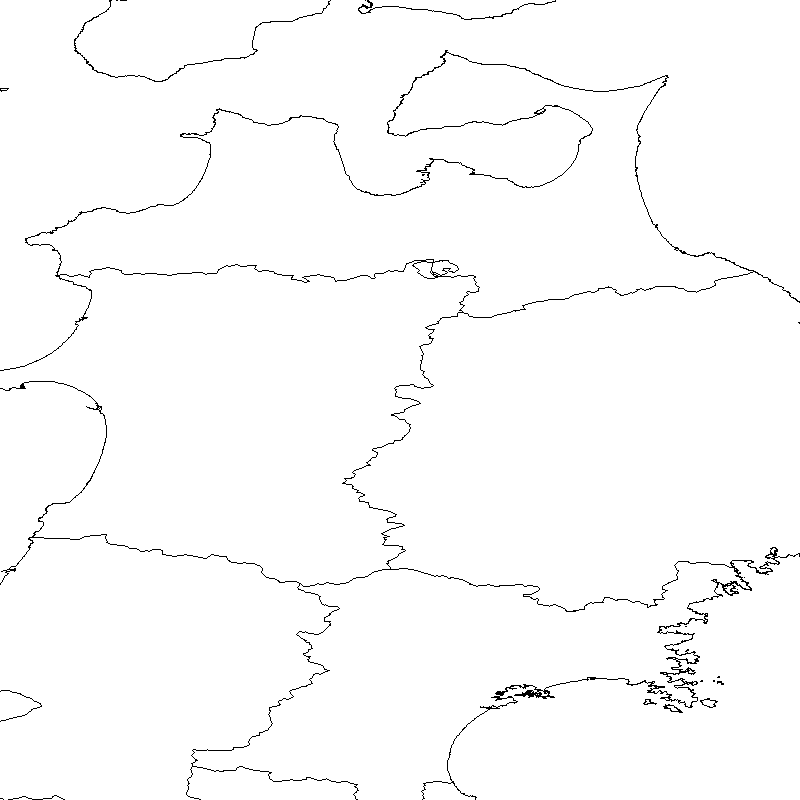
\includegraphics[scale=0.1]{touhoku.png}
	}
	\caption{Touhoku.}
	\label{touhoku}
\end{figure}

\paragraph{East Japan} Is the region that is related with the east coast of Japan. It is the most different area, because it has earthquakes that happened both in land or in the sea. It was in this region that the 9.0 $M_w$ earthquake happened. Its coordinates are 37 North, 140 West, with 1600 bins. Each bin covers an area of approximately 100km$^2$. \\


	\begin{figure}[H]
		\centering
		\fbox{
			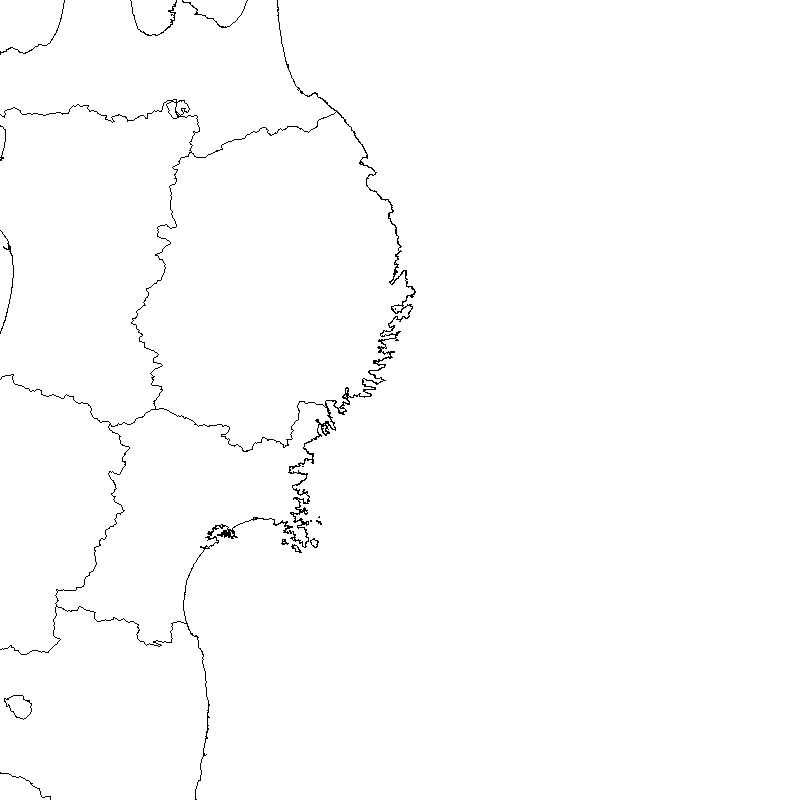
\includegraphics[scale=0.1]{coast.png}
		}
		\caption{East of Japan.}
		\label{eastJapan}
	\end{figure}

\section{Depth Histogram of Earthquakes}

%TODO: add ref
The patterns of earthquakes are dependent of the depth. We wanted to explore the relation between the depth of the earthquakes and how would our models behave on those situations.\\

In Figure~\ref{histogramQuakes}, it is possible to understand that most of the earthquakes happened with depths smaller or equal to 100 km. The earthquakes deeper than 100 km are fewer and more distant, as it is in the same Figure.\\

\begin{figure}[!htb]
	\centering
	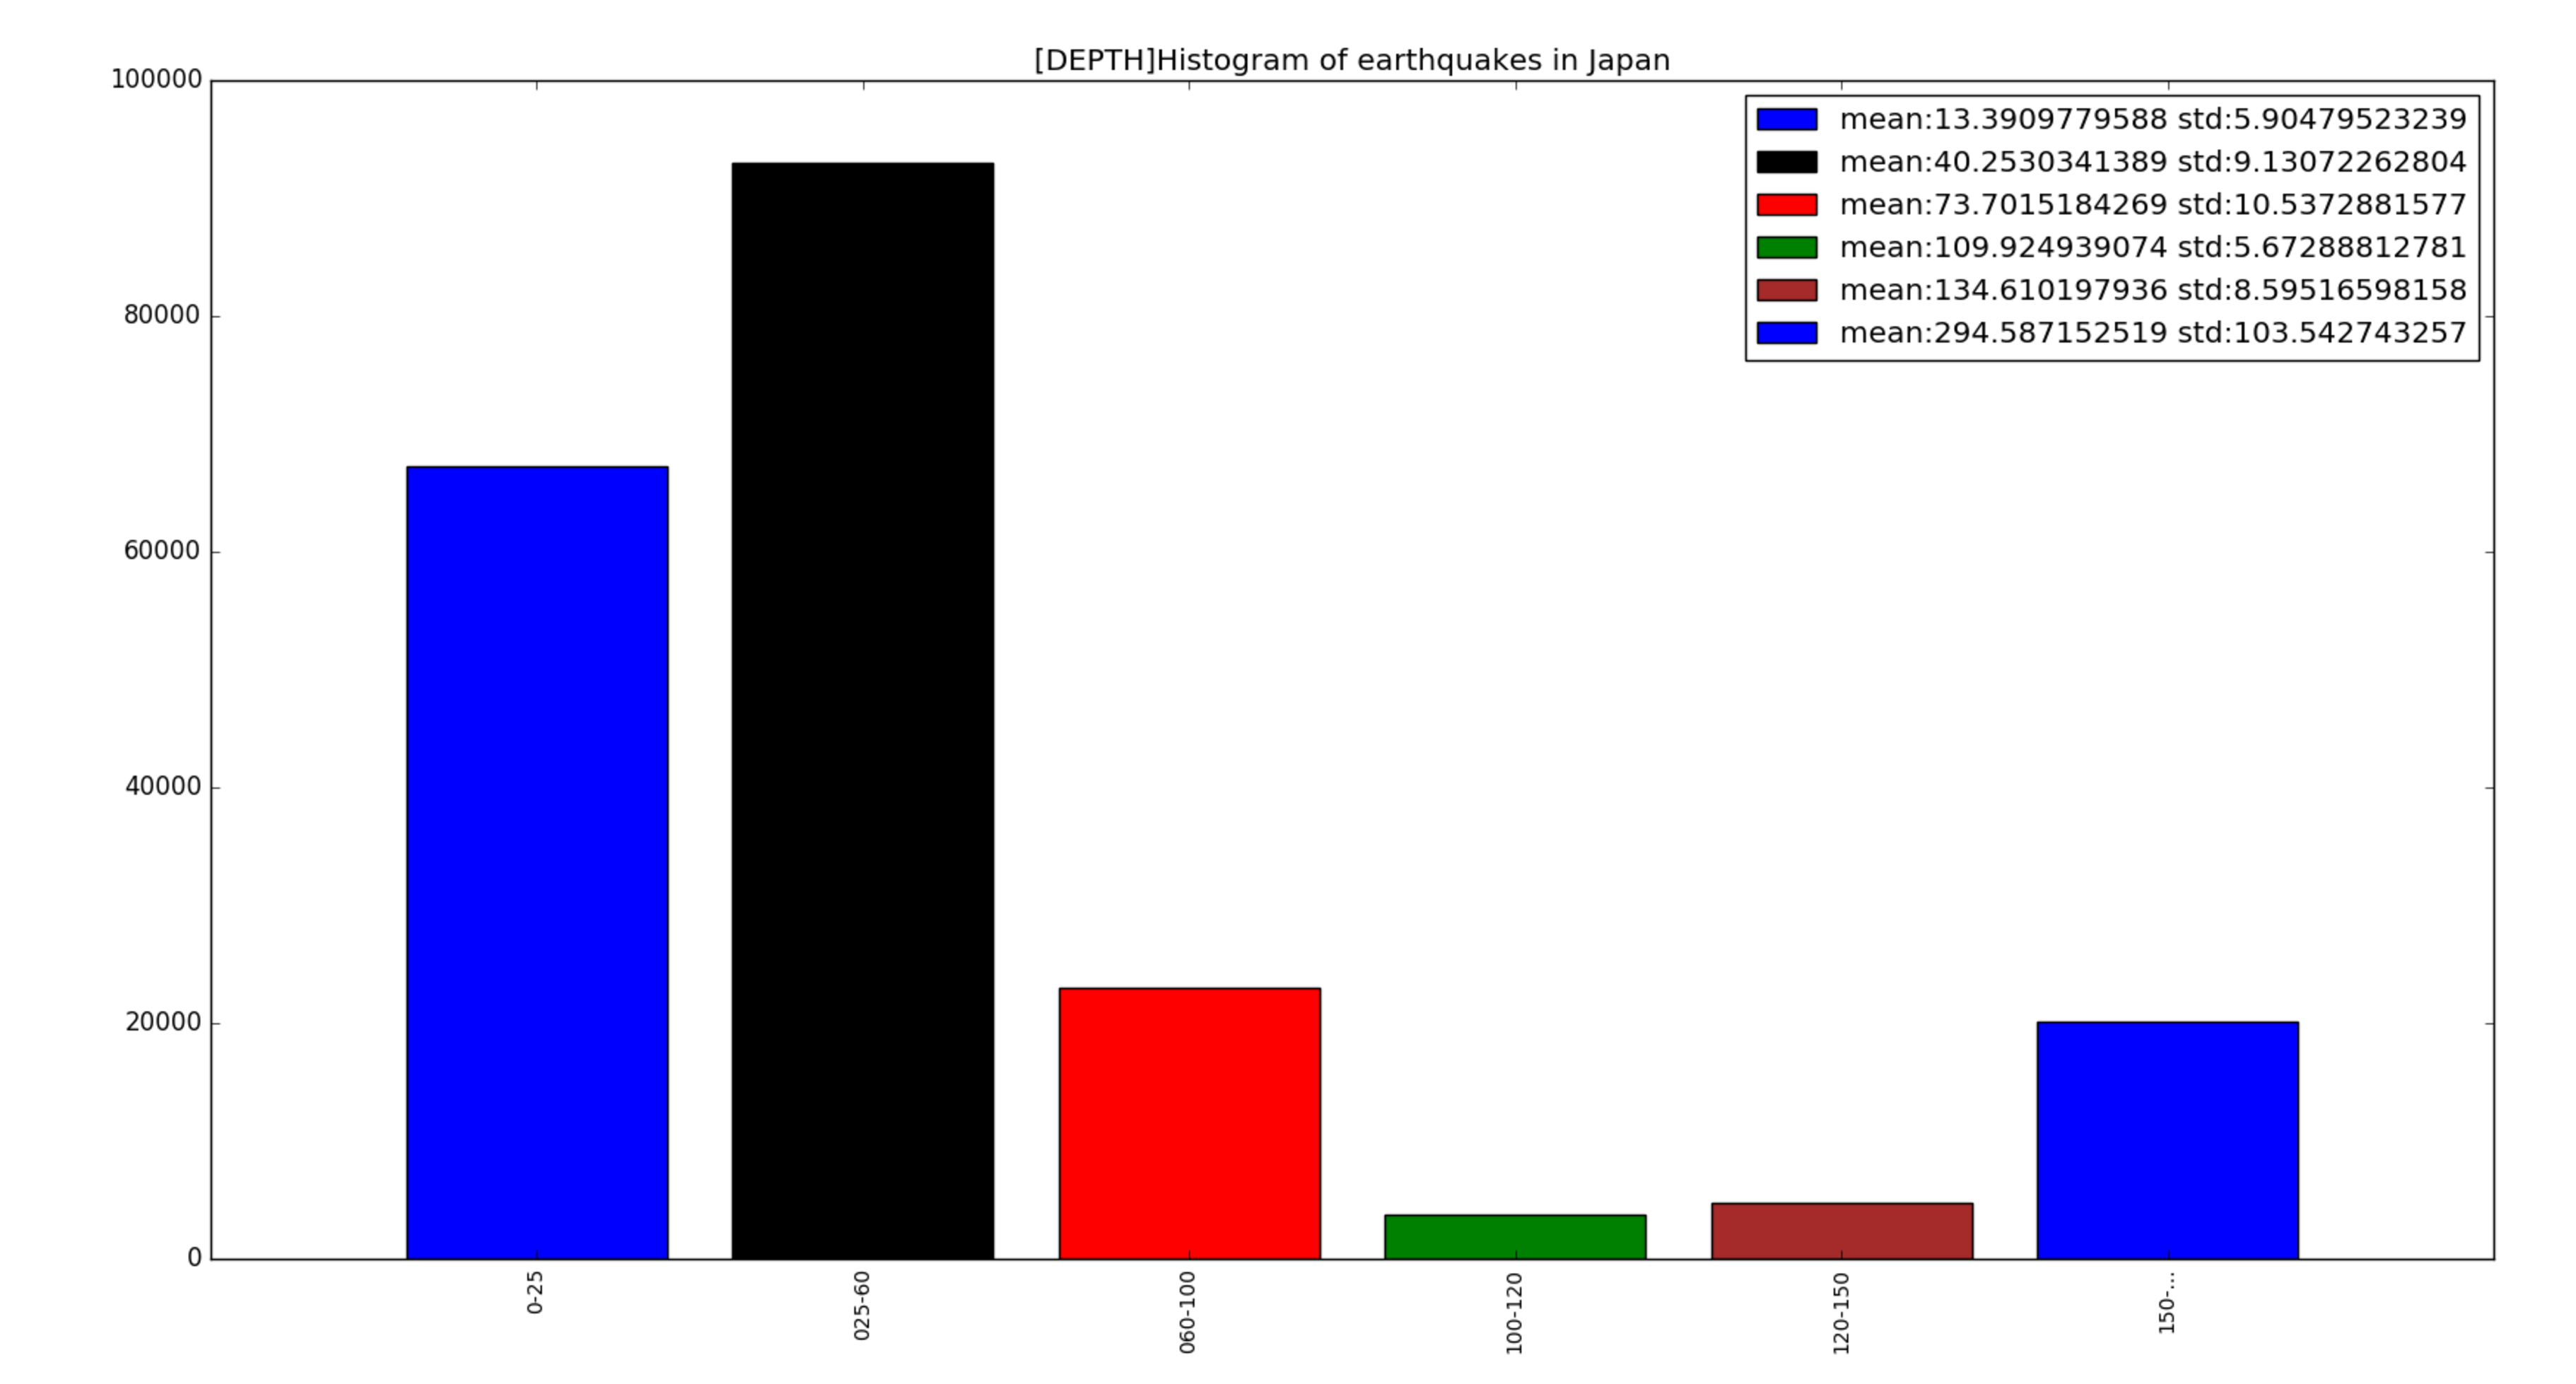
\includegraphics[scale=0.25, left]{detphsNew.pdf}
	\caption{Depth Histogram of earthquakes.}
	\label{histogramQuakes}
\end{figure}

The reason we decided to groups as: earthquakes shallow than 25 km, shallow than 60 km and shallow than 100 km. This is because shallow quakes are considered to be more independent quakes~\cite{yamanaka1990scaling}.

\subsection{Main-shocks and After-shocks - Clustering}\label{Clustering}

In the last Chapter,~\ref{chapter4}, we explained that we have two kinds of models, the ones that only consider after-shocks and those that consider both main-shocks and after-shocks. Therefore, it is needed to isolate, to classify the quakes into one of these two groups.\\

The question is how should it be done. The simplest way, is to select earthquakes with magnitude above 3.0 in the Richter Scale and then to consider those as the main-shocks The distribution of earthquakes in after this selection is exemplified in the Figure~\ref{quakesKanto}.\\

\begin{figure}[!htb]
	\centering
	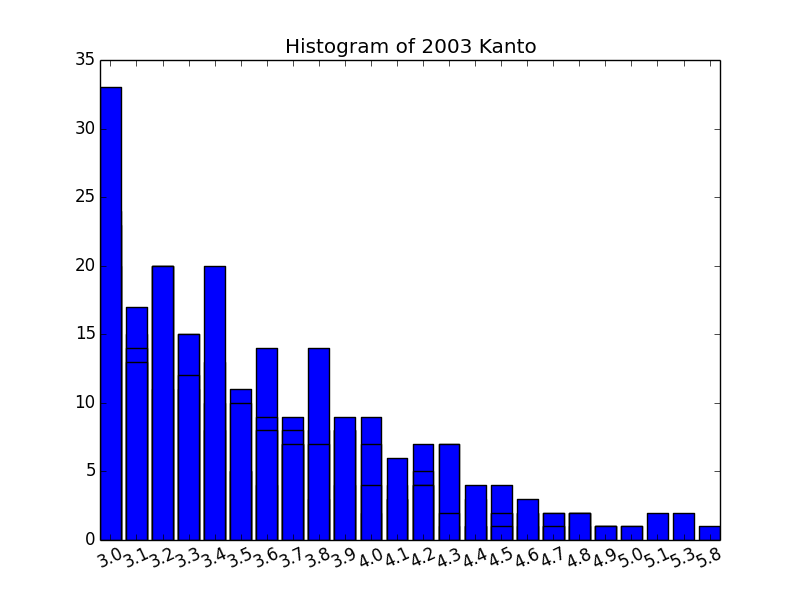
\includegraphics[scale=0.5]{Magnitude2003Kanto.png}
	\caption{Histogram of earthquakes stronger than 3.0 in the Richter Scale in Kanto}
	\label{quakesKanto}
\end{figure}

%TODO: check what info I need to use from Gabriel's
The problem with this simple idea is: if a big main-shock happens and it triggers some after-shocks with magnitude higher than 3.0 in the Richter Scale it would be considered as a main-shock To avoid this problem we used two methods proposed in the literature: Window Methods and the Single-Link Cluster. For more information about those methods~\ref{van2012seismicity}.\\ 